\refstepcounter{section}
\section*{Lecture 23: Interior Solution (contd.)}
\addcontentsline{toc}{section}{Lecture 23: Interior Solution (contd.)}
In the previous section, we started discussing about the interior solutions for Einstein's equation. Let us now start with the equation for $r$,
$$G_{rr} = 8\pi G \ST_{rr} \implies \frac{1}{r^2}\qty[1 - e^{2\nu} + 2r\phi' ] = 8\pi G P e^{2\nu}$$
as $u_{r}$ component of the four-velocity is zero. Multiplying the above equation by $r^2$ and $e^{-2\nu}$ we get
$$(\underbrace{e^{-2\nu}-1}_{-\frac{2G\SM(r)}{r}}) + 2r\dv{\phi}{r} e^{-2\nu} = 8\pi G r^2\rho$$
Multiplying further by $r$ and simplifying, we have the final expression
\begin{equation}\label{eqn:TOV2}
    \boxed{\dv{\phi}{r} = G\frac{\qty[\SM(r)+4\pi r^3P]}{r(r-2G\SM(r))}}
\end{equation}
\begin{tcolorbox}[colframe=black, colback=lime!20!white, boxrule=1.5pt, arc=4pt]
Show that for the interior metric, $\nabla_\mu \ST^{\mu\nu} = 0$ leads to,
\begin{equation}\label{eqn:TOV3}
    \dv{P}{r} = -(\rho+P)\dv{\Phi}{r}
\end{equation}
\end{tcolorbox}
\noindent
\textit{Proof.} Let us first calculate the stress-energy tensor assuming the perfect fluid condition,
$$\vartriangleright\ST^{rr} = Pe^{-2\nu}\quad \vartriangleright \ST^{\theta\theta} = \frac{P}{r^2}\quad \vartriangleright \ST^{\phi\phi} = \frac{P}{r^2\sin^2\theta} \quad \vartriangleright \ST^{tt} = (P+\rho)e^{-2\Phi} -Pe^{-2\Phi} = \rho e^{-2\Phi}$$
Then applying the conservation criterion for the stress-energy tensor, we have
\begin{align*}
    0 = \nabla_\mu \ST^{\mu r} &= \partial_\mu\ST^{\mu r} + \chris{r}{\mu}{\sigma}\ST^{\mu\sigma} + \chris{\mu}{\mu}{\sigma}\ST^{\sigma r}\\
    &=\partial_r \qty(Pe^{-2\nu}) + \chris{r}{r}{r}\ST^{rr}+\chris{r}{\theta}{\theta}\ST^{\theta\theta}+\chris{r}{\phi}{\phi}\ST^{\phi\phi}+\chris{r}{t}{t}\ST^{tt}+\chris{\mu}{\mu}{r}\ST^{rr}
\end{align*}
Expanding the last term we get the following
$$\chris{\mu}{\mu}{r} = \chris{t}{t}{r} +\chris{r}{r}{r}+\chris{\theta}{\theta}{r} +\chris{\phi}{\phi}{r} = \Phi' + \nu'+\frac{1}{r}+\frac{1}{r} =    \Phi' + \nu'+\frac{2}{r}$$
Then, we putting all these together we get
\begin{align*}
    0 &=\partial_r \qty(Pe^{-2\nu}) + \qty(P\nu'e^{-2\nu}) + \qty(-re^{-2\nu}\frac{P}{r^2}) + \qty(-r\sin^2\theta e^{-2\nu}\frac{P}{r^2\sin^2\theta})+ \Phi' e^{2(\Phi - \nu)} \rho e^{-2\Phi}+\qty(\Phi'+\nu' + \frac{2}{r})Pe^{-2\nu}\\
    &=\qty(\dv{P}{r}-2\nu'P)e^{-2\nu} + \qty(P\nu'e^{-2\nu}) -\qty(e^{-2\nu}\frac{2P}{r})+ \Phi' e^{-2\nu} \rho+\qty(\Phi'+\nu' + \frac{2}{r})Pe^{-2\nu}\\
    &=\qty{\qty(\dv{P}{r}-\cancel{2\nu'P}) + \cancel{\qty(P\nu')} -\cancel{\qty(\frac{2P}{r})}+ \Phi'  \rho+\qty(\Phi'+\cancel{\nu'} + \cancel{\frac{2}{r}})P}e^{-2\nu}\\
    &=\qty{\dv{P}{r} +\Phi'(\rho+P)}e^{-2\nu}
\end{align*}
We have used the form of the Christoffel symbols from the code given in the appendix. Eq. \ref{eqn:TOV1}, \ref{eqn:TOV2} and \ref{eqn:TOV3} are together called the \textit{Tolman-Oppenheimer-Volkoff} equations which are used to model an isotropic, spherically symmetric body in hydrostatic equilibrium.
\subsection{Newtonian Analogy}
Consider a spherical mass $M$ and radius $R$ with a thin shell at distance $r$, which collapses due to gravitational attraction. Then, we can write the \textit{mass-balance} equation as,
$$\dv{M(r)}{r} = 4\pi r^2 \rho(r)$$
where $\rho(r)$ is the density at distance $r$. We can also write the hydrostatic equilibrium equation, for which we need to balance the pressure gradient force.
\begin{figure}[H]
    \centering 


\tikzset{every picture/.style={line width=0.75pt}} %set default line width to 0.75pt        

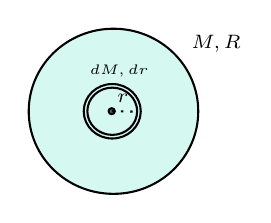
\begin{tikzpicture}[x=0.75pt,y=0.75pt,yscale=-1,xscale=1]
%uncomment if require: \path (0,232); %set diagram left start at 0, and has height of 232

%Shape: Ellipse [id:dp9120616292548687] 
\draw  [fill={rgb, 255:red, 80; green, 227; blue, 194 }  ,fill opacity=0.24 ] (222,109.34) .. controls (222,87.37) and (240.28,69.56) .. (262.84,69.56) .. controls (285.4,69.56) and (303.68,87.37) .. (303.68,109.34) .. controls (303.68,131.31) and (285.4,149.12) .. (262.84,149.12) .. controls (240.28,149.12) and (222,131.31) .. (222,109.34) -- cycle ;
%Shape: Ellipse [id:dp5508841063539507] 
\draw  [fill={rgb, 255:red, 0; green, 0; blue, 0 }  ,fill opacity=0.52 ] (260.51,109.3) .. controls (260.51,110.1) and (261.18,110.74) .. (261.99,110.74) .. controls (262.81,110.74) and (263.47,110.1) .. (263.47,109.3) .. controls (263.47,108.5) and (262.81,107.86) .. (261.99,107.86) .. controls (261.18,107.86) and (260.51,108.5) .. (260.51,109.3) -- cycle ;
%Straight Lines [id:da5551042710853338] 
\draw  [dash pattern={on 0.84pt off 2.51pt}]  (261.99,109.3) -- (273.71,109.5) ;
%Shape: Donut [id:dp36921431792355186] 
\draw   (250.25,109.34) .. controls (250.25,103.05) and (255.62,97.95) .. (262.25,97.95) .. controls (268.87,97.95) and (274.24,103.05) .. (274.24,109.34) .. controls (274.24,115.63) and (268.87,120.72) .. (262.25,120.72) .. controls (255.62,120.72) and (250.25,115.63) .. (250.25,109.34)(248.51,109.34) .. controls (248.51,102.09) and (254.66,96.21) .. (262.25,96.21) .. controls (269.83,96.21) and (275.98,102.09) .. (275.98,109.34) .. controls (275.98,116.59) and (269.83,122.46) .. (262.25,122.46) .. controls (254.66,122.46) and (248.51,116.59) .. (248.51,109.34) ;

% Text Node
\draw (263.26,99.46) node [anchor=north west][inner sep=0.75pt]  [font=\scriptsize]  {$r$};
% Text Node
\draw (299,71.4) node [anchor=north west][inner sep=0.75pt]  [font=\scriptsize]  {$M,R$};
% Text Node
\draw (250,85.4) node [anchor=north west][inner sep=0.75pt]  [font=\tiny]  {$dM,dr$};


\end{tikzpicture}


\end{figure}
Balancing the pressure, we have the hydrostatic equilibrium,
$$4\pi r^2(P(r+\dd r) - P(r)) = -\frac{GM(r)\dd M}{r^2}\implies \dv{P}{r} = -\frac{GM(r)\rho}{r^2}$$
Now, from the Newtonian potential we can write
$$\Phi\tund{N} = -\frac{GM}{r} \implies \dv{\Phi\tund{N} }{r} = \frac{GM}{r^2}$$
\textcolor{red}{understand what is happening?}
\subsection{Boundary Matching}
We had previously stated also, that the metric should be continuous across the boundary from which we had obtained $\SM(R) = M$ where $M$ is the mass of the star. We can also match the component of $g_{tt}$ from which we get
$$e^{2\Phi} = \qty(1-\frac{2GM}{R}) \implies \Phi(R) = -\frac{GM}{R} \quad \text{if $\Phi(R)\ll 1$}$$